\documentclass[
	fontsize=12pt,
	paper=a4,
	twoside=false,
	numbers=noenddot,
	plainheadsepline,
	toc=listof,
	toc=bibliography
]{scrartcl}

\usepackage[german,ngerman]{babel} % Silbentrennung
%\usepackage[T1]{fontenc} % Ligaturen, richtige Umlaute im PDF 
\usepackage[utf8]{inputenc}% UTF8-Kodierung für Umlaute usw

\usepackage[round]{natbib}

\usepackage{amssymb,amsmath}

\usepackage{placeins}
\usepackage{float}
\restylefloat{table}

\restylefloat{figure}
\usepackage{subfigure} 

\usepackage{tikz}
\usepackage{color,colortbl}

\usepackage{hyperref}

\usepackage{placeins}

% Literaturverzeichnis
\usepackage{natbib}

% Absätze
\setlength{\parindent}{0pt}

\usepackage{graphicx}

\begin{document}
%----------------------------------------------------------------------------------------------------
%----------------------------------------------------------------------------------------------------
\section{Klassisches Modell}
%----------------------------------------------------------------------------------------------------
%----------------------------------------------------------------------------------------------------
\begin{table}[htbp]
\centering
\begin{tabular}{|c|c|c|c|c|}
\hline 
	Lattice    & $L(2,1)$   & $L(3,2,1)$ & $L(4,3,2,1)$ & $L(5,4,3,2,1)$ \\ \hline 
	Hexagonal  & $5$        & $9$        & $19$         & $30$           \\ 
($24$ Knoten)  & $0.16$sec  & $0.95$sec  & $47.09$sec   & $3123.74$sec   \\ \hline
			   
	Triangular& $8$	        & $18$        &  $32$            &    \\ 
($23$ Knoten) & $0.91$sec   & $573.48$sec &  $934550$sec     &    \\ \hline
			  
	Square    &  $6$	    &  $11$       & $25$         &    \\ 
($25$ Knoten) & $0.63$sec   &  $1.72$sec  & $8619.05$sec & \\ \hline
\end{tabular}
\caption{ Ergebnisse des klassischen Modells angewendet aud drei Type der Gridgraphen} 
\label{Table:T0}
\end{table}

\begin{table}[htbp]
\centering
\begin{tabular}{|c|c|c|c|c|}
\hline 
	Lattice    & $L(2,1)$   & $L(3,2,1)$ & $L(4,3,2,1)$ & $L(5,4,3,2,1)$ \\ \hline 
	
	Hexagonal  & $5$        & $9$        & $20$          & $30$           \\ 
    ($30$ Knoten)  & $0.26$sec  & $1.86$sec  & $491.37$sec   & $23509.7$sec   \\ \hline
			   
	Triangular & $8$	 & $18$         & $18$        &    \\ 
    ($30$ Knoten)  & $1.71$sec  & $9830.71$sec & $9807.55$sec&    \\ \hline
			  
	Square    & $6$	         & $11$         & $25$             &    \\ 
    ($30$ Knoten) & $1.08$sec   & $2.36$sec    & $20124.8$sec     & \\ \hline

\end{tabular}
\caption{ Ergebnisse des klassischen Modells angewendet aud drei Type der Gridgraphen} 
\label{Table:T0}
\end{table}


\newpage
%----------------------------------------------------------------------------------------------------
%----------------------------------------------------------------------------------------------------
\section{$L(3,2)$ vs $L(2,1)$}
%----------------------------------------------------------------------------------------------------
%----------------------------------------------------------------------------------------------------


\begin{table}[htbp]
\centering
\begin{tabular}{|c|c|c|}
	\hline
	 
	 Lattice                & $L(2,1)$  & $L(3,2)$     \\ \hline 
	 Hexagonal (24 nodes)   & 5	 & 9  \\ 
			        & $0.16$sec	 & $0.42$sec  \\ \hline
	 Triangular (23 nodes)  & 8	 & 16  \\ 
			        & $0.90$sec	 & $17.92$sec  \\ \hline
	 Square (25 nodes)      & 6	 & 11  \\ 
			        & $0.63$sec	 & $2.24$sec  \\ \hline
	 Hexagonal (30 nodes)   & 5	 & 9  \\ 
			        & $0.25$sec	 & $1.04$sec  \\ \hline
	 Triangular (30 nodes)  & 8	 & 16  \\ 
			        & $2.59$sec	 & $19.23$sec  \\ \hline
	 Square (30 nodes)      & 6	 & 11  \\ 
			        & $1.07$sec	 & $1.30$sec  \\ \hline			       

\end{tabular}
\caption{$L(3,2)$ vs $L(2,1)$} 
\label{Table:TG3}
\end{table}

\FloatBarrier 

%----------------------------------------------------------------------------------------------------
\newpage
%----------------------------------------------------------------------------------------------------	
%----------------------------------------------------------------------------------------------------
\section{Modelle}
%----------------------------------------------------------------------------------------------------
%----------------------------------------------------------------------------------------------------


\begin{table}[htbp]
\centering
\begin{tabular}{|c|c|c|c|c|c|}
\hline 
	Lattice   & $ f(x)=3-x$  & $L(2,1)$   & & $f(x)=4-x$    & $L(3,2,1)$  \\ \hline 
	
	Hexagonal & $6.41699$	  & $5$        & & $16.6243$     & $9$         \\ 
			  & $4.57$sec     & $0.16$sec  & & $5577.68$sec  & $0.95$ sec   \\ \hline

	Triangular& $9.78029$ 	  & $8$         & & $21.9068$     & $18$         \\ 
			  & $38.62$sec    & $0.91$sec   & & $368958$ sec  & $573.48$sec  \\ \hline
			  
	Square    & $8.63494$	  & $6$         & & $19.9067$     & $11$   \\ 
			  & $15.34$sec    & $0.63$sec  & & $153587$sec    & $1.72$sec \\ \hline
\end{tabular}
\caption{ Ergebnisse für L(2,1), L(3,2,1) im klassischen Fall und Funktion $f(x)=3-x$, $f(x)=4-x$ im Fall der
	reelwertigen Labeling.} 
\label{Table:T1}
\end{table}

\FloatBarrier	

\begin{figure}[hb]
    \subfigure[$L(2,1)$ Labeling, optimal value $8.78029$]{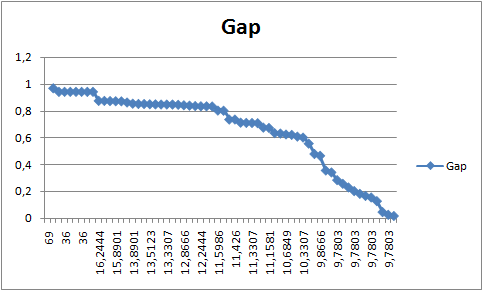
\includegraphics[width=0.49\textwidth]{L21.png}}
    \subfigure[$L(3,2,1)$ Labeling, optimal value $21.9068$]{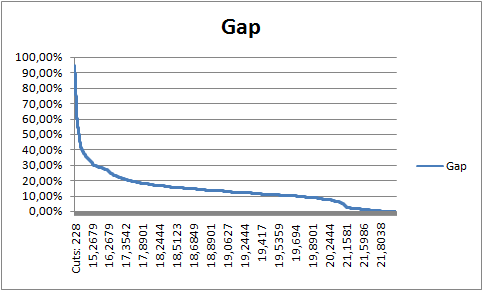
\includegraphics[width=0.49\textwidth]{L321.png}}
\caption{Evolution of the LB in case of triangular lattice graph and real number labeling}
\end{figure} 




\FloatBarrier	

\newpage
%----------------------------------------------------------------------------------------------------
%----------------------------------------------------------------------------------------------------
\section{Treppenfunktion}
%----------------------------------------------------------------------------------------------------
%----------------------------------------------------------------------------------------------------
\begin{table}[htbp]
\centering
\begin{tabular}{|c|c|c|c|c|c|}
\hline 
	Lattice   & $ f(x)=3-x$  & $L(2,1)$   & & $f(x)=4-x$    & $L(3,2,1)$\\ \hline 
	
	Hexagonal &  $5$	     & $5$         & & $9$            & $9$       \\ 
			  &  $2.18$sec   & $0.16$sec   & & $3.8$sec       & $0.95$sec \\ \hline
			  
	Triangular& $8$	         & $8$        & & $18$          & $18$        \\ 
			  & $27.34$sec   & $0.91$sec  & & $4599.13$sec  & $573.48$sec  \\ \hline
			  
	Square    &  $6$	     & $6$        & & $11$          & $11$        \\ 
			  &  $22.95$sec  & $0.63$sec  & & $10.17$sec    & $1.72$sec   \\ \hline
\end{tabular}
\caption{ Ergebnisse für L(2,1), L(3,2,1) im klassischen Fall und Treppenfunktion im Fall der
	reelwertigen Labeling.} 
\label{Table:T2}
\end{table}


\FloatBarrier	

\newpage
%----------------------------------------------------------------------------------------------------
%----------------------------------------------------------------------------------------------------
\section{Verbessern der Laufzeit}
%----------------------------------------------------------------------------------------------------
%----------------------------------------------------------------------------------------------------

\subsection{Bescränkung der Konstanten $M$}
%----------------------------------------------------------------------------------------------------
	\begin{table}[htbp]
	\centering
	\begin{tabular}{|c|c|c|c|c|c|}
	\hline 
	Lattice   & $f(x)=3-x$(new) & $f(x)=3-x$(old) & & $f(x)=4-x$ (new) & $f(x)=4-x$(old)\\ \hline 

	Hexagonal & $6.41699$	    & $6.41699$       & & $16.6243$        & $16.6243$   \\ 
			  & $5.19$sec      & $4.57$sec       & & $6283.5$sec       &  $5577.68$  \\ \hline
			  
	Triangular& $9.78029$      & $9.78029$       & & $21.9068$        & $21.9068$   \\ 
			  & $30.29$sec     & $38.62$sec      & & $211144.36$sec      & $368958$sec  \\ \hline
	
	Square    & $8.63494$       & $8.63494$       & & $19.9067$        & $19.9067$   \\ 
			  & $23.72$sec      & $15.34$sec      & & $84990.2$sec     & $153587$sec  \\ \hline
	\end{tabular}
	\caption{ Der Vergleich der Laufzeit des vorherigen Modells und des Modells mit den zusatzlichen Beschränkungen auf die Konstanten M} 
	\label{Table:T31}
	\end{table}
\FloatBarrier	

%----------------------------------------------------------------------------------------------------	
\subsection{Bescränkung von $\alpha$}
%----------------------------------------------------------------------------------------------------
	\begin{table}[htbp]
	\centering
	\begin{tabular}{|c|c|c|c|c|c|}
	\hline 
	Lattice   & $f(x)=3-x$(new)   & $f(x)=3-x$(old) & & $f(x)=4-x$ (new)  & $f(x)=4-x$(old)\\ \hline 
	
	Hexagonal & $6.41699$	       & $6.41699$       & & $16.6243$         & $16.6243$   \\ 
			  & $13.28+135.43=$    & $4.57$sec       & & $337947+410468=$  & $5577.68$sec\\
			  & $148.71$sec        &                 & & $748414$sec       &  \\ \hline			
			    
	Triangular& $9.78029$          & $9.78029$       & & $21.9068$        & $21.0968$\\ 
			  & $447.24+883.27=$   & $38.62$sec      & & $ $              & $368958$sec\\ 
			  & $ 1330.51$sec      &                 & & $ $              & \\ \hline			  
	
	Square    & $8.63494$         & $8.63494$       & & $19.9067$        & $19.9067$   \\ 
			  & $118.89+198.25=$  &  $15.34$sec      & & $ $              & $153587$ sec \\ 
			  & $317.14$sec       &                 & & $ $              &  \\ \hline			  
	\end{tabular}
	
	\caption{ Ansatz der binären Suche für die Bestimmung oberer und unterer Schranken für $\alpha$ } 
	\label{Table:T31}
	\end{table}
\FloatBarrier	

%----------------------------------------------------------------------------------------------------
\subsection{Teilgrephen}	
%----------------------------------------------------------------------------------------------------
\begin{table}[htbp]
\centering
\begin{tabular}{|c|c|c|c|}
	\hline 
	
	Hexagonal Lattice & $d(x)=3-x$  & $d(x)=4-x$   & nConstraints \\ \hline 
	Der ganze Graph	  &  6.41699	 & 16.6243      &              \\ 
 			          &  $4.57$sec  & $5577.68$sec & $601$\\ \hline
 			          
	Teilgraphen & & &\\\hline
	Sechsecke mit der Seitenlänge $1$      & $4.33$sec & $15952.01$sec   & $608$\\ \hline
	Sechsecke mit der Seitenlänge $1$, $2$	& $4.35$sec	 & $8879.65$sec & $609$\\ \hline
	Trapez                                 & $6.75$sec & $7104.64$sec  & $614$ \\ \hline

\end{tabular}
\caption{Untersuchung der Teilgraphen, Fall der Gridgraphen aus der Sechsecken.} 
\label{Table:TG1}
\end{table}
	
\begin{table}[htbp]
\centering
\begin{tabular}{|c|c|c|c|}
		\hline 
		
		Triangular Lattice  & $d(x)=3-x$    & $d(x)=4-x$   & nConstraints \\ \hline 
		Der ganze Graph     & $9.78029$	 & $21.9068$    &              \\ 
			                & $38.62$sec    & $368958$sec  & $553$        \\ \hline
			                
		Teilgraphen & & &\\\hline
		Dreiecke mit der Seitenlänge $1$         & $21.03$sec	 & $294858.83$sec    & $581$\\ \hline
		Dreiecke mit der Seitenlänge $1$,$2$,$3$ & $37.21$sec	 & $543555.6$sec    & $589$\\ \hline
		Sechsecke mit der Seitenlänge $1$        & $36.65$sec  & $151160.25$ sec   & $560$ \\ \hline

\end{tabular}
\caption{Untersuchung der Teilgraphen, Fall der Gridgraphen aus der Dreiecken.}
\label{Table:TG2}
\end{table}
	
	
\begin{table}[htbp]
\centering
\begin{tabular}{|c|c|c|c|}
	\hline
	 
	 Square Lattice       & $d(x)=3-x$  & $d(x)=4-x$   & nConstraints  \\ \hline 
	 Der ganze Graph	   & 8.63494	 & 19.9067      &               \\ 
			              & $15.34$sec	 & $153587$sec  & $651$\\ \hline
			              
	Teilgraphen & & &\\ \hline
	Vierecke mit der Seitenlänge $1$                         & $24.32$sec	& $182766.41$sec & $667$\\ \hline
	Vierecke mit der Seitenlänge $1$,$2$,$3$ ohne Überlappen & $24.56$sec   & $265454.68$sec & $672$\\ \hline
	Vierecke $1\times 2$                                     & $33.18$sec   & $killed$       & $659$\\ \hline

\end{tabular}
\caption{Untersuchung der Teilgraphen, Fall der Gridgraphen aus der Vierecken.} 
\label{Table:TG3}
\end{table}
%----------------------------------------------------------------------------------------------------





\end{document}